\documentclass[report.tex]{subfiles}
\graphicspath{ \subfix{./images/} \subfix{./graphs/} }
\begin{document}
\section{Milestone 2: Implement the data structures and database}

\subsubsection{Implementation and testing}

I decided to create a second project called Algorithm Dynamics.Core to separate the UI code and the core code. This allows me to organize the codebase more cleanly and allows me to run unit tests on the core code.

When developing the core code, I decide not to integrate it with the UI right away, since it is very inefficient in testing and debugging. Instead, I will write unit tests for each function, test everything in isolation, and then integrate the core code with the UI when it is ready.

I decided to create the model and the database structure at the same time, so that I can make sure any change to the data model will be saved correctly into the database, preventing any data inconsistency between the runtime and the database.

I decide to use SQLite\cite{sqlite} as the database since it is a small, fast and lightweight database suitable for local data storage. To access the database, I use Microsoft.Data.Sqlite\cite{microsoft:docs:sqlite} database to send my query commands to the local database.

First, I create a test table to test the workflow. Under Algorithm Dynamics.Core.Helpers namespace, I create a class DataAccess. I decide to make it public since it needs to be accessed to set the physical location of the database. I decide to make it static since it is essentially a collection of helper functions that depend on each other, but no instance needs to be created to call them. I decide to set it to a partial class since I intend to split functions that handle different data models into different files, so each file only contains a part of the class.

\begin{minted}{csharp}
using Microsoft.Data.Sqlite;
using System.IO;

namespace Algorithm_Dynamics.Core.Helpers
{
    public static partial class DataAccess
    {
    }
}
\end{minted}

I set up a private attribute \code{DbPath}, which stores the physical location of the database. And a function \code{InitDatabase}, which takes in a string, and init the database at that location.

\begin{minted}{csharp}
/// <summary>
/// Store the physical loaction of the database.
/// Use <see cref="InitializeDatabase(string)"/> to initialize the value.
/// </summary>
private static string DbPath;

/// <summary>
/// Initialize the database at the <see cref="dbPath"/> given.
/// Execute CREATE TABLE commands.
/// </summary>
/// <param name="dbPath"></param>
public static void InitializeDatabase(string dbPath)
{
}
\end{minted}

\begin{minted}{csharp}
public static void InitializeDatabase(string dbPath)
{
    // Save the DbPath
    DbPath = dbPath;

    // Create a new database if not exist
    if (!File.Exists(dbPath))
    {
        File.CreateText(dbPath).Dispose();
    }

    // Create tables
    using (SqliteConnection db = new(ConnectionString))
    {
        db.Open();

        string tableCommand =
            @"CREATE TABLE IF NOT EXISTS MyTable 
            (
                Primary_Key INTEGER PRIMARY KEY,
                Text_Entry TEXT
            );";
        SqliteCommand createTable = new(tableCommand, db);

        createTable.ExecuteNonQuery();
    }
}
\end{minted}

TODO: Implementation

\subsubsection{Integration}

I then need to integrate the core code with the UI.

On the HomePage, I need to implement the random problem button and the recommendations.

\begin{minted}{csharp}
private void InitializeQAItems()
{
    // ...    
    QAItems.Add(new QuickAccessItem("Random Problem", Symbol.Shuffle, () =>
        {
            // Get all problems from the database
            List<Problem> problems = Problem.All;

            // Generate a random index
            var random = new Random();
            int randomIndex = random.Next(problems.Count);

            // Get the corresponding problem
            Problem problem = problems[randomIndex];

            // Navigate to coding page with the problems as parameters
            App.NavigateTo(typeof(CodingPage), Tuple.Create(problem, problems));
        }));
    // ...
}

/// <summary>
/// Generate Recommendation from database.
/// </summary>
private void InitializeRecItems()
{
    RecItems.Clear();
    // Generate recommend problems
    var problems = Problem.All;
    for (int i = 0; i < problems.Count && i < 4; i++)
    {
        var problem = problems[i];
        RecItems.Add(new RecommendItem(problem.Name, $"{problem.DifficultyAsString} | {problem.TagAsString}", () => { App.NavigateTo(typeof(CodingPage), Tuple.Create(problem, Problem.All)); }));
    }
    // If no item, hide the title
    if (RecItems.Count == 0)
    {
        RecommendTextBlock.Visibility = Visibility.Collapsed;
    }
    else
    {
        RecommendTextBlock.Visibility = Visibility.Visible;
    }
}
\end{minted}

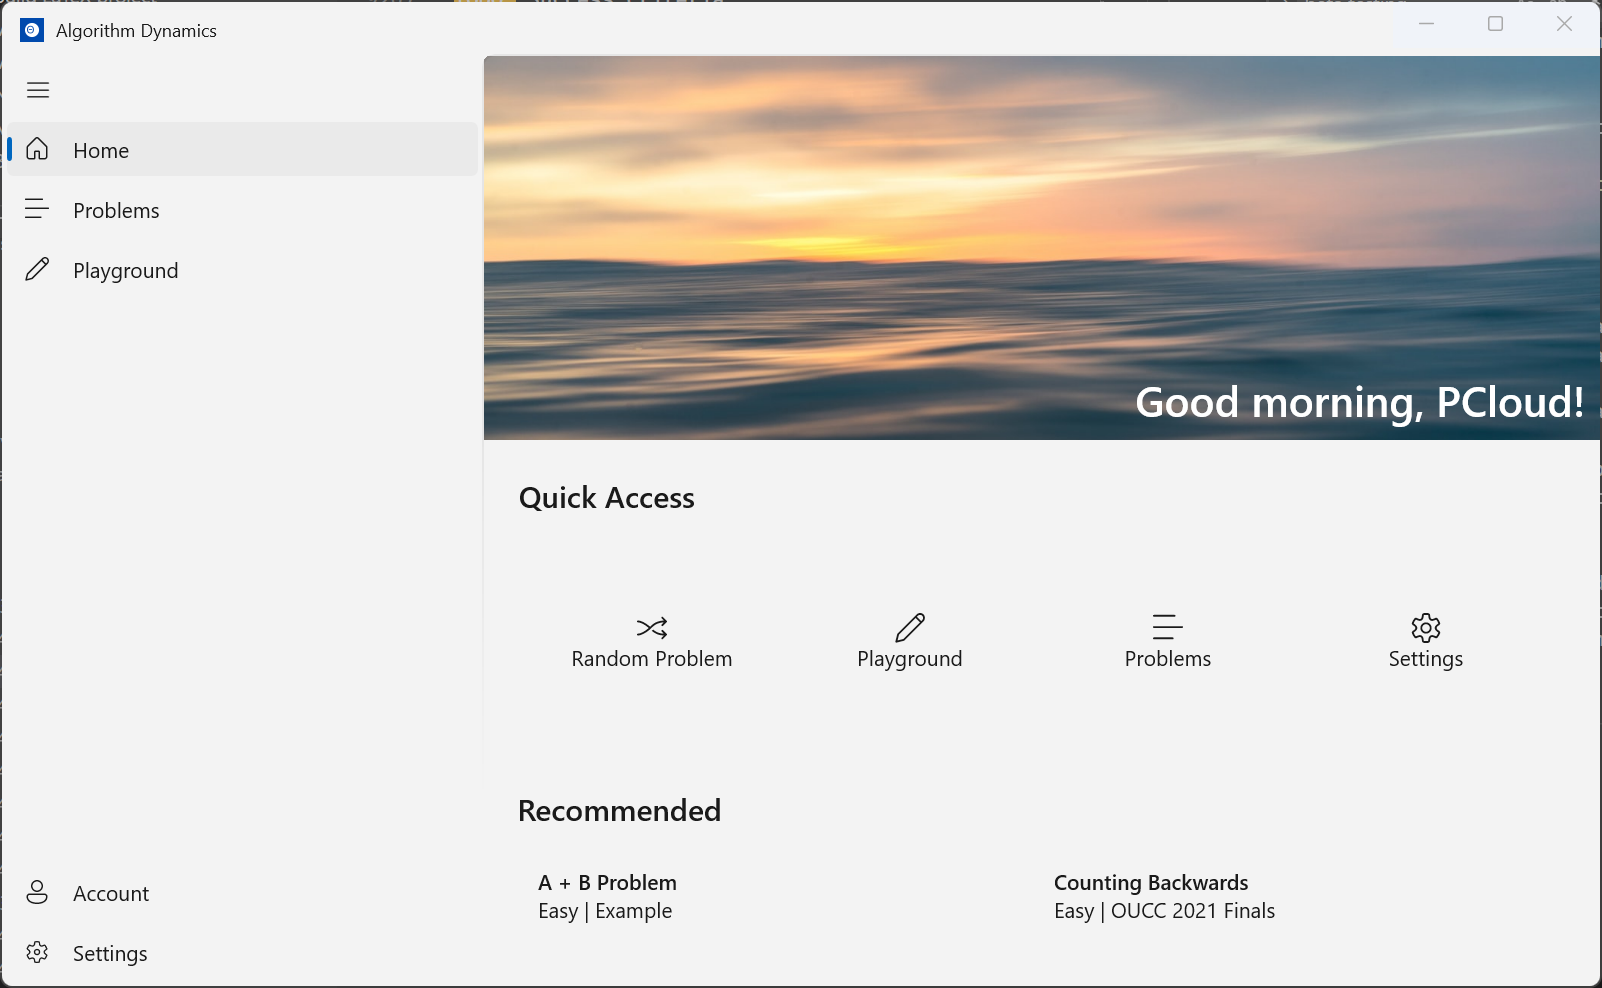
\includegraphics[width=\textwidth, height=\textheight, keepaspectratio]{HomePage-Final}

Now, when I click the random problem button or the recommendations button, I am navigated to the correct problem correctly.

TODO: ProblemsPage

TODO: CreateNewProblemPage

TODO: CreateNewProblemListPage

TODO: CodingPage

TODO: AccountPage

\end{document}